\textbf{(CAP-COLUNI 2024 -- Q17)} Durante uma gincana de Matemática no CAp-Coluni, os estudantes tiveram que dançar, movimentando os braços, de acordo com gráficos de funções matemáticas pré-selecionadas. A estudante Júlia se apresentou e, de maneira correta, fez os movimentos com os braços indicados, ordenadamente, nas figuras abaixo.

\begin{center}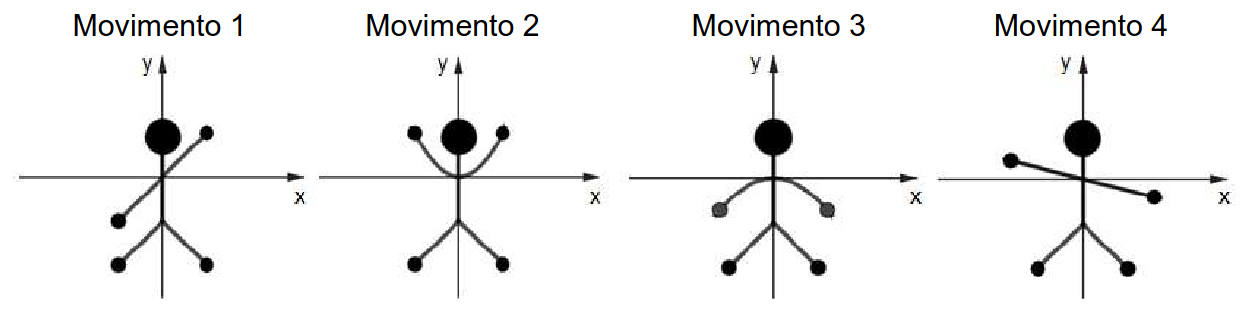
\includegraphics[width=0.98\linewidth]{static/simulados/coluni/latex-figs/2024-Q17.png}\end{center}

Considere que as posições dos braços indicadas acima ilustrem partes de gráficos de funções matemáticas de 1º e 2º graus. A alternativa que contém as funções que melhor representam, ordenadamente, os movimentos dos braços de Júlia, durante a dança na gincana de Matemática, é:



\begin{enumerate}
	\item $y=x$, $y=x^2$, $y=-\frac{x^2}{2}$ e $y=-\frac{x}{4}$.
	\item $y=2x$, $y=2x^2+1$, $y=-\frac{x^2}{2}+1$ e $y=-x$.
	\item $y=x+1$, $y=\frac{x^2}{2}$, $y=-x^2-1$ e $y=-x-1$.
	\item $y=\frac{x}{2}$, $y=2x^2$, $y=-x^2$ e $y=x$.
\end{enumerate}
